\section{Estrutura}

\subsection{Definição das Aletas}
As aletas exercem um papel fundamental na estabilidade aerodinâmica de foguetes. Sua principal função é deslocar o centro de pressão (CP) para uma posição abaixo do centro de massa (CM), garantindo assim a correção de ângulos de ataque indesejados durante o voo. Para cumprir esse papel de forma eficaz, é essencial que as aletas sejam construídas com materiais que combinem baixa densidade, elevada rigidez e espessura reduzida, de modo a minimizar o peso e a interferência aerodinâmica. 

Ademais, a resistência mecânica do material é um fator determinante, uma vez que o foguete está sujeito a impactos significativos durante o pouso. Após analisar diferentes opções, optamos pelo poliestireno de alto impacto (PSAI) para a fabricação das aletas, por oferecer um bom equilíbrio entre rigidez, peso e resistência ao impacto. 

Outros materiais, como o PVC rígido ou plásticos leves de engenharia, também foram considerados, entretanto o PSAI se mostrou mais adequado para o projeto. A escolha inadequada do material poderia levar a deformações durante o voo ou fraturas nas aletas, comprometendo a trajetória e a reutilização do foguete. 

Dessa forma, a definição do material das aletas considerou não apenas o desempenho aerodinâmico, mas também a integridade estrutural ao longo de múltiplos lançamentos, garantindo que o projeto atenda aos requisitos de estabilidade e durabilidade 

\subsection{Definição da Base de Lançamento}

\subsubsection{Estabilidade Estrutural}
A concepção estrutural da base de lançamento prioriza a estabilidade como um critério fundamental, influenciando diretamente a precisão e segurança de sua operação. A decisão de uma configuração com base de apoio quadrada, materializada em tubos de PVC, demonstrou-se suficiente e superior em relação a geometrias alternativas, como a de tripé, sob diversos princípios da estática. 

A geometria quadrada proporciona uma área de contato com o solo significativamente maior, otimizando a distribuição das cargas estáticas do foguete e das cargas dinâmicas causadas pelo lançamento. Tal configuração minimiza a suscetibilidade ao tombamento, assegurando que o centro de gravidade do sistema foguete-base permaneça contido no perímetro de apoio, mesmo sob a influência de perturbações externas, como rajadas de vento ou o impulso do lançamento. Adicionalmente, o projeto contempla a possibilidade de ancoragem ao solo ou a uma placa de madeira por meio de grampos, o que eleva substancialmente a resistência a deslocamentos indesejados. 

Em contrapartida, uma estrutura do tipo tripé, embora apresente estabilidade intrínseca em superfícies irregulares, possui uma área de projeção da base de apoio potencialmente menor, o que a torna mais vulnerável a momentos fletores induzidos por forças laterais. 

A decisão em favor do modelo de base quadrada é reforçada pela consideração da estabilidade dimensional. O design incorpora um elemento de reforço estrutural, um braço de suporte, cuja função é garantir a rigidez do sistema, prevenindo a deflexão do tubo de lançamento sob a carga do foguete. Esta deformação, comum em estruturas mais simples, comprometeria a manutenção do ângulo de lançamento de 45°, impactando negativamente a precisão do alcance. 

Conclui-se, portanto, que a geometria quadrada adotada não apenas otimiza a estabilidade contra o tombamento, mas também preserva a integridade estrutural necessária para a consistência do ângulo de lançamento, um parâmetro crítico para o controle de trajetória requerido pelo projeto. 

\subsubsection{Mecânica do Lançamento e Ajuste Angular}
A dinâmica do lançamento de projéteis é regida por princípios da mecânica clássica, nos quais o ângulo de lançamento funciona como uma variável determinante do alcance horizontal. Para uma velocidade de ejeção constante, a trajetória parabólica descrita pelo foguete atinge seu alcance máximo quando o ângulo de lançamento é de 45 graus em relação ao plano horizontal. Qualquer desvio deste ângulo pode resultar em uma redução do alcance potencial. 

Esta decisão estratégica simplifica a complexidade mecânica da base, elimina fontes potenciais de erro associadas a juntas móveis e garante a constância do ângulo em todos os lançamentos. Tal abordagem permite que o controle da trajetória e do alcance seja exclusivo pela variação da pressão de lançamento, conforme previsto na estratégia de operação. 

\subsubsection{Materiais Estruturais}
A escolha do Policloreto de Vinila (PVC) como material principal justificada por um conjunto favorável de propriedades. A principal vantagem do PVC é sua notável facilidade de manuseio e montagem, que demanda apenas ferramentas simples, como serras manuais, lixas e adesivos específicos para a união dos componentes. Adicionalmente, o baixo custo e a ampla disponibilidade comercial destes componentes de PVC asseguram a viabilidade econômica do projeto. 

Outra opção seria materiais metálicos, que ofereçam resistência mecânica superior, porém implicariam em um aumento na complexidade de fabricação e nos custos. A madeira, por sua vez, apresentaria maior massa e suscetibilidade à degradação por umidade, um fator relevante no contexto de foguetes com propulsão de água. 

A capacidade de carga do PVC, ainda que inferior à dos metais, é adequada e segura para a pressão e as cargas dinâmicas envolvidas no lançamento, sendo um material padrão em projetos educacionais e competições, como a Mostra Brasileira de Foguetes (MOBFOG). 

\subsection{Desenho Técnico}

A elaboração de um desenho técnico, especialmente por meio de modelagem 3D, é uma etapa significativa antes da construção da estrutura de um projeto. Possuir uma representação de como o foguete e sua plataforma de lançamento de PVC serão permite visualizar todo o projeto de forma clara e precisa, antecipando a aparência e disposição dos componentes. 

 Além disso, o desenho técnico atua como um guia definitivo para a construção, onde cada etapa segue uma norma conforme descrita. A visualização inicial por meio do desenho técnico permite encontrar diferenças, erros de tamanho e incompatibilidades entre as peças antes mesmo da montagem propriamente dita. Ao corrigir essas discrepâncias antecipadamente, é possível economizar materiais e reduzir o tempo necessário para alterações durante os testes. 

Com a ajuda do software CATIA, foi possível fazer a representação 3D do modelo do foguete, junto à sua base. Foram utilizados os tamanhos reais das peças esolhidas para a confecção do modelo. Algumas peças, para ajudar na fidedignidade do projeto de CAD como a vida real, foram retiradas diretamente do site TraceParts, com as devidas proporções (diâmetro de 20mm, ou 3/12”). A unidade adotada nas figuras do desenho técnico é mm.

\begin{center}
    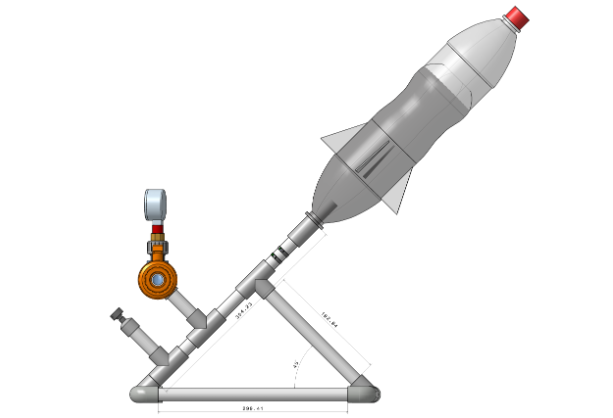
\includegraphics[width=0.5\textwidth]{figuras/vista_lateral.png}
    \\\textbf{Figura 1:} Vista lateral do desenho técnico.
\end{center}

\begin{center}
    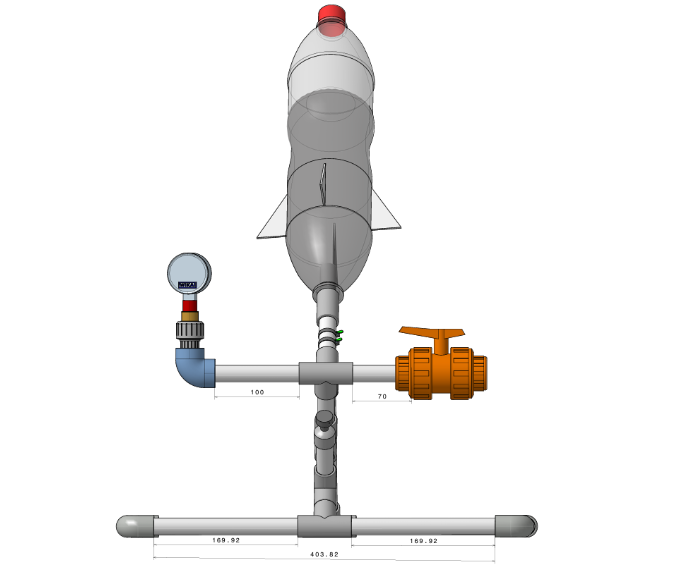
\includegraphics[width=0.5\textwidth]{figuras/vista_frontal.png}
    \\\textbf{Figura 2:} Vista frontal do desenho técnico.
\end{center}

\begin{center}
    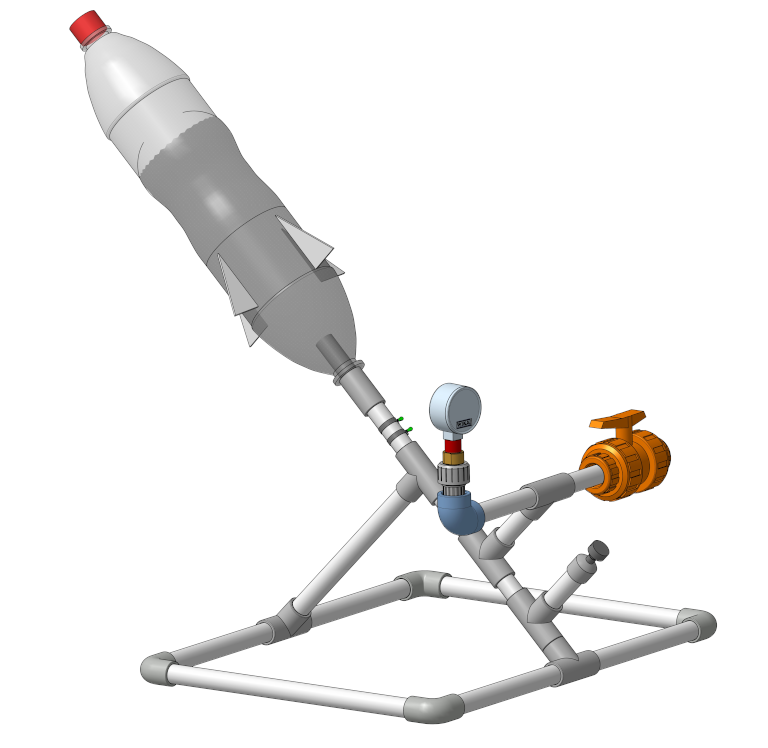
\includegraphics[width=0.5\textwidth]{figuras/vista_isometrica.png}
    \\\textbf{Figura 3:} Vista isométrica do desenho técnico.
\end{center}

% -------------------------------------------------------------------------------------
% revisar estes testes e colocar na lista de testes gerais
% -------------------------------------------------------------------------------------

%\section{Testes}
%
%Para garantir que o material escolhido para a estrutura do foguete resistisse aos impactos gerados durante o lançamento, realizamos testes experimentais simulando quedas controladas. 
%
%Para compor a fuselagem do foguete, consideramos duas opções: a garrafa PET convencional e a retornável. Para fins comparativos, unimos ambas em um único corpo, conforme ilustrado na figura abaixo. 
%
%\begin{center}
%    \includegraphics[width=0.5\textwidth]{figuras/estrutura_teste.png}
%    \\\textbf{Figura 4:} Estrutura do teste.
%\end{center}
%
%Com aproximadamente 400 gramas de água adicionadas ao interior do foguete, a estrutura foi liberada de uma altura significativa. A cada teste, alternamos a extremidade voltada para o solo, a fim de avaliar a resistência ao impacto de cada material. 
%
%\begin{center}
%    \includegraphics[width=0.5\textwidth]{figuras/representacao_teste.png}
%    \\\textbf{Figura 5:} Representação do teste.
%\end{center}
%
%Inicialmente, a garrafa PET retornável foi considerada para a construção da estrutura, por apresentar maior espessura e rigidez. No entanto, observou-se que esse tipo de PET não possui elevada tenacidade, ou seja, tende a romper-se de forma frágil sem apresentar deformação prévia. Além disso, o material perde resistência estrutural com o tempo e o uso repetido. 
%
%Após algumas quedas, a garrafa PET retornável não resistiu e quebrou, como demonstrado na figura abaixo. Em contrapartida, a garrafa PET convencional demonstrou desempenho superior, absorvendo o impacto com deformações localizadas que não comprometeram a integridade da estrutura. 
%
%\begin{center}
%    \includegraphics[width=0.5\textwidth]{figuras/garrafa_quebrada.png}
%    \\\textbf{Figura 6:} Garrafa PET retornável após o teste.
%\end{center}
